\setchapterpreamble[u]{\margintoc}
\chapter{Statistical Approach to Drop Formation}
\labch{dropstat}


\section{Monte Carlo Approach}



% determination of droplet diameter and volume 



\section{Millimeter Scale Ensembles}

We turn our attention towards slender ligaments whose widths are of the 
order of millimeters, a scale at which a multitude of fragmentation phenomena
\sidenote{Some examples of fragmentation at this length scale involve ligaments
generated by drop splashes on different substrates, secondary atomization of raindrops etc. 
}
take place, that are more or less visible to the naked eye.
In particular, for air-water systems (20 degree Celsius) the millimeter length 
scale corresponds to $Oh \sim O(10^{-2})$, where $Oh$ is the Ohnesorge number
based on the characteristic length scale of the ligaments. 
The characterization of our corrugated ligament setup using the set of adimensional
(e.g. \eqref{base_params}) numbers as discussed in the previous chapter is extended 
to describe our ensemble of ligaments, such that the exact set of parameters
correspond to a unique point in the phase space $\Phi$ of all possible combinations. 
The coalescences that intermittently occur after the initial breakup phase of 
the thread-like structure not only change the number of drops, but also impact the 
mean and dispersion of the size distribution due to the increase in the number of drops that 
are significantly larger than the width of the ligament of origin.   
This aspect of temporal dependence of the drop sizes corresponding to a particular ligament ensemble
is taken into account by specifying the time at which the statistics are recorded. 
Thus, our droplet ensembles associated with the millimeter scale ligaments can be uniquely described 
by a combination of the time $T$ and $\Phi_0$, where

\begin{align}
	\Phi_0 \equiv \left( Oh=10^{-2}, K=2\pi, \epsilon=1.0, \Lambda=50 \right). 
\end{align}

The definitions of the adimensional groups are identical to that used
in the previous chapter, hence are not repeated.
Statistical descriptions of the drop sizes are commonly carried out using
particular probability density functions (PDF) defined as follows 



\begin{align}
	\text{Gaussian : } \quad P\left( x ; \mu , \sigma \right) &= 
	\frac{1}{\sigma \sqrt{2\pi}} \textrm{exp}\left[-\frac{1}{2}\left(\frac{x - \mu}{\sigma}\right)^2\right] \label{gauss},\\
	\text{Log-Normal : } \quad P\left( x ; \mu , \sigma \right) &= 
	\frac{1}{x \sigma \sqrt{2\pi}} \textrm{exp}\left[-\frac{1}{2}\left(\frac{\log x - \mu}{\sigma}\right)^2\right] \label{log_normal},\\
	\text{Gamma : } \quad P\left( x ; n,k \right) &= 
	\frac{k^{n}}{\Gamma(n)} x^{n-1} \textrm{exp}\left(-k x\right) \label{gamma}, 
\end{align}

where $x$ is the variable (diameter, volume etc) in question. 
The Gamma distribution can be rearranged so that $x$ represents
the variable rescaled by its mean ($n / k$), which becomes 

\begin{align}
	P\left( x ; n \right) = \frac{n^{n}}{\Gamma(n)} x^{n-1} \textrm{exp}\left(-n x\right) . 
\end{align}

The rescaling of variable results renders the function dependent solely 
on the parameter $n$, identical to the form first used in \cite{vill_2}
to represent the distribution of the normalized diameter.  
At the large size limit of the distributions, the leading order terms 
scale as $P(x) \sim \textrm{exp}(-x^2)$ for the Gaussian, $P(x) \sim \textrm{exp}(- \log x)$ for 
the Log-Normal and finally $P(x) \sim \textrm{exp}(- x)$ in case of the Gamma function. 
In essence, out of the three density functions, the Guassian predicts the lowest frequency of
rare events (very large drops), the Log-Normal predicts the highest frequency whereas
the Gamma function prediction is somewhere in between the other two. 

\begin{marginfigure}[-1cm]
\centering
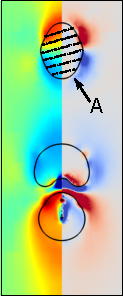
\includegraphics{plots/drop_stats/diameter_compute.pdf}
\caption{The shaded area $A$ represented by the dotted and dashed lines
	is used to estimate the diameter of the droplet in question.
	The resulting diameter is computed as $D = \sqrt{4A/\pi}$,
	and the corresponding volume is given by $V = \pi D^3/6$.
	} 
\label{dia_compute}
\end{marginfigure}

Another important aspect to consider is the bin-width of the 
histograms used to construct the probability distributions. 
There are several choices regarding the criteria used to determine the optimal bin-width, 
taking into consideration the size, variability and skewness of the underlying data set. 
In in interest of simplicity, we restrict our focus to histograms with uniform bin-width. 
In order to ascertain the dependence (if any) of the distribution on the number of bins  
(uniform size), we use $4$ different estimators, the open source implementations of which
can be found in the Numpy library \cite{numpy}.
The simplest of the four estimators selects the number 
of bins as the square root of the sample size.
Another estimator is also based solely on the size of the dataset, 
but the number of bins scales as the cube root of the data size.  
A more robust estimator that takes into account the variability in the dataset
is the Freedman Diaconis estimator, in which the bin width is proportional to the 
inter quartile range, and inversely proportional to the cube root of the data size. 
Finally, we also use an improved version of the Sturges estimator, that performs 
well for non-normal datasets due to the fact that it takes into account the skewness. 

In the subsequent sections, we present a statistical picture of the drop sizes generated 
from our ligament ensemble $\Phi_0$, where the sample size is of the order of $64,000$.
The droplet data is primarily recorded on slow time scales, so that the data reflects 
a considerable amount of coalescences after the initial destabilization of the ligaments. 
In order to extract the diameter and volumes of the drops generated in our axisymmetric
simulations, we for the commonly used area based estimation (see Fig. \ref{dia_compute}).


\subsection*{Diameter Distributions}

Figures \ref{t1_dia_bins} and \ref{t2_dia_bins} illustrate the probability distributions
of the normalized droplet diameter corresponding to $T=15$ and $T=30$ respectively. 
The diamters are normalized using the means of the associated samples. 
The bin widths are always based on the properties of the largest sample.
As one can observe, there are fewer drops in the largest sample at $T=30$ 
compared to the largest sample at $T=30$, due to the additional coalescences.  
The drop diameters are found to be more or less symmetrically distributed about the mean,
although there is an small peak at the lower end of the dis.
The choice of binning criteria does not seem to have any noticable effect on the 
overall shape of the distribution, regardless of the size of the sample $N$.   
A Guassian probability density function \eqref{gauss} appears to be a good 
approximation to the underlying distribution.
It is important to note that the Gaussian curve is not fitted to the heights of the 
histogram bins, instead it is plotted on top of the distributions using the mean and 
variance corresponding to the largest sample size, therefore rendering it independent
of the choice of bin-width and free from any additional fitting parameters.  


\begin{figure*}
\centering
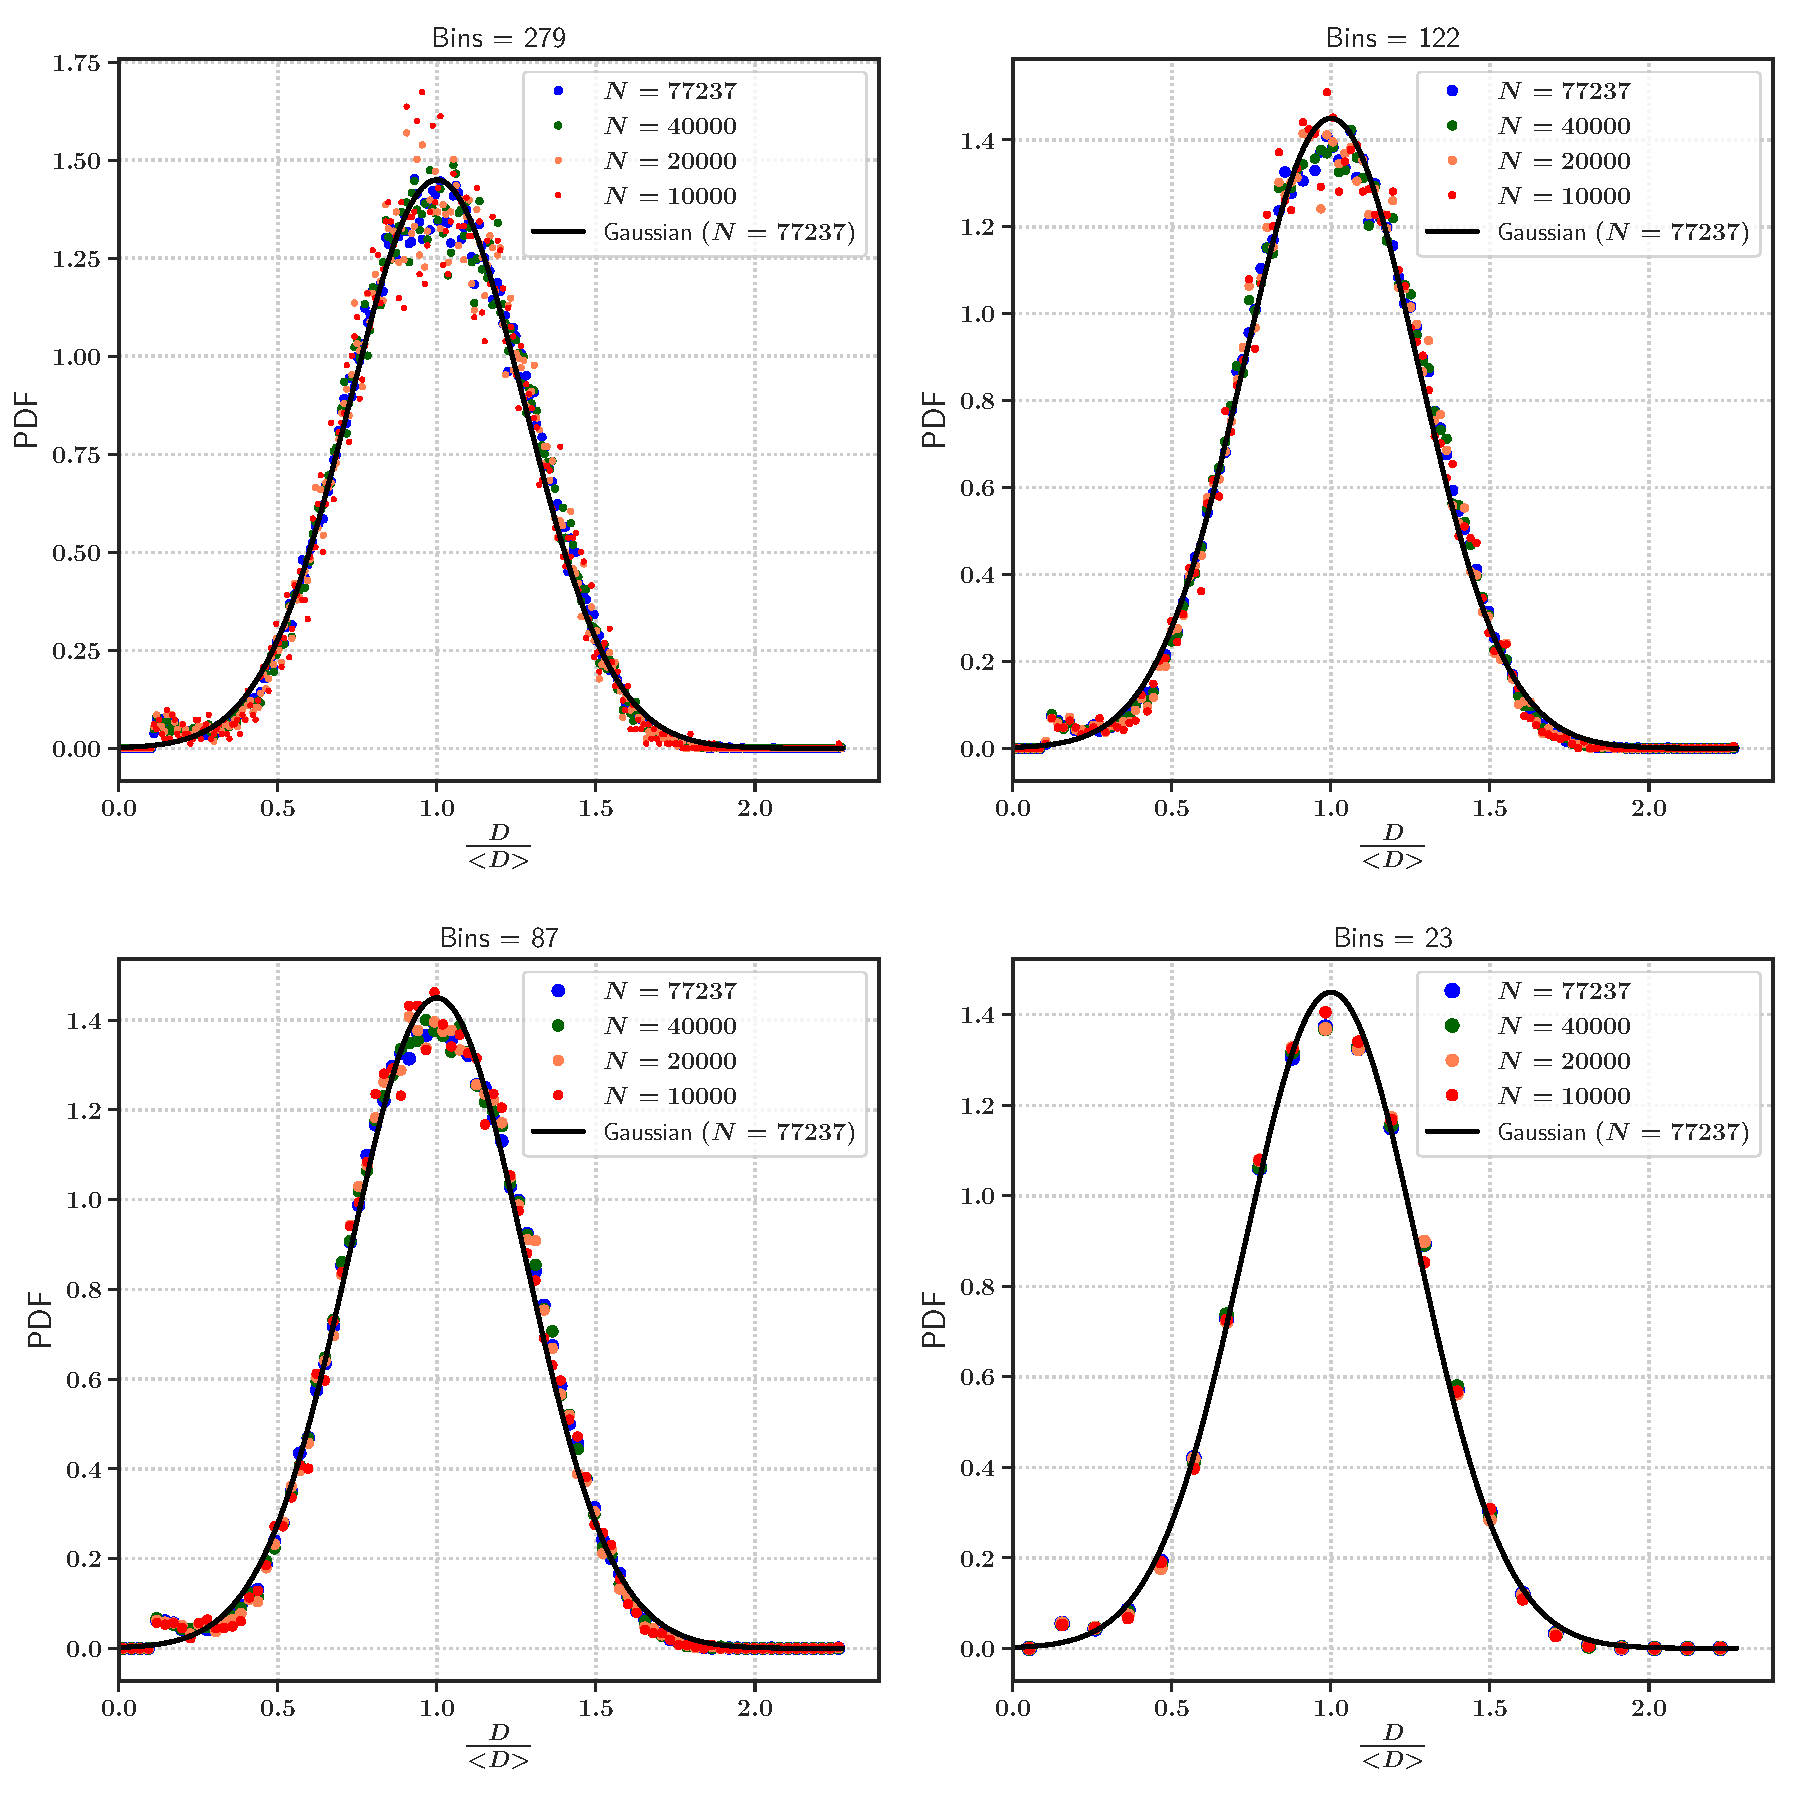
\includegraphics{plots/drop_stats/short_time_diameter_bins.pdf}
\caption{Probability distribution functions of the droplet diameter at time $T = 15$. 
The ensemble is characterized by $\Phi_0 \equiv \left( Oh = 10^{-2}, K = 2\pi , \varepsilon = 1.0 , \Lambda = 50 \right)$. 
The diameters are normalized by the mean of the corresponding sample.  
The distributions are generated using datasets corresponding to four different sample sizes, 
including four different choices of (uniform) bin width. 
The Gaussian functions are characterized by the mean and variance of the original dataset, 
hence they are plotted alongside the histograms instead of being fitted to the bin heights.
	}
\label{t1_dia_bins}
\end{figure*}

% long time scales



\begin{figure*}
\centering
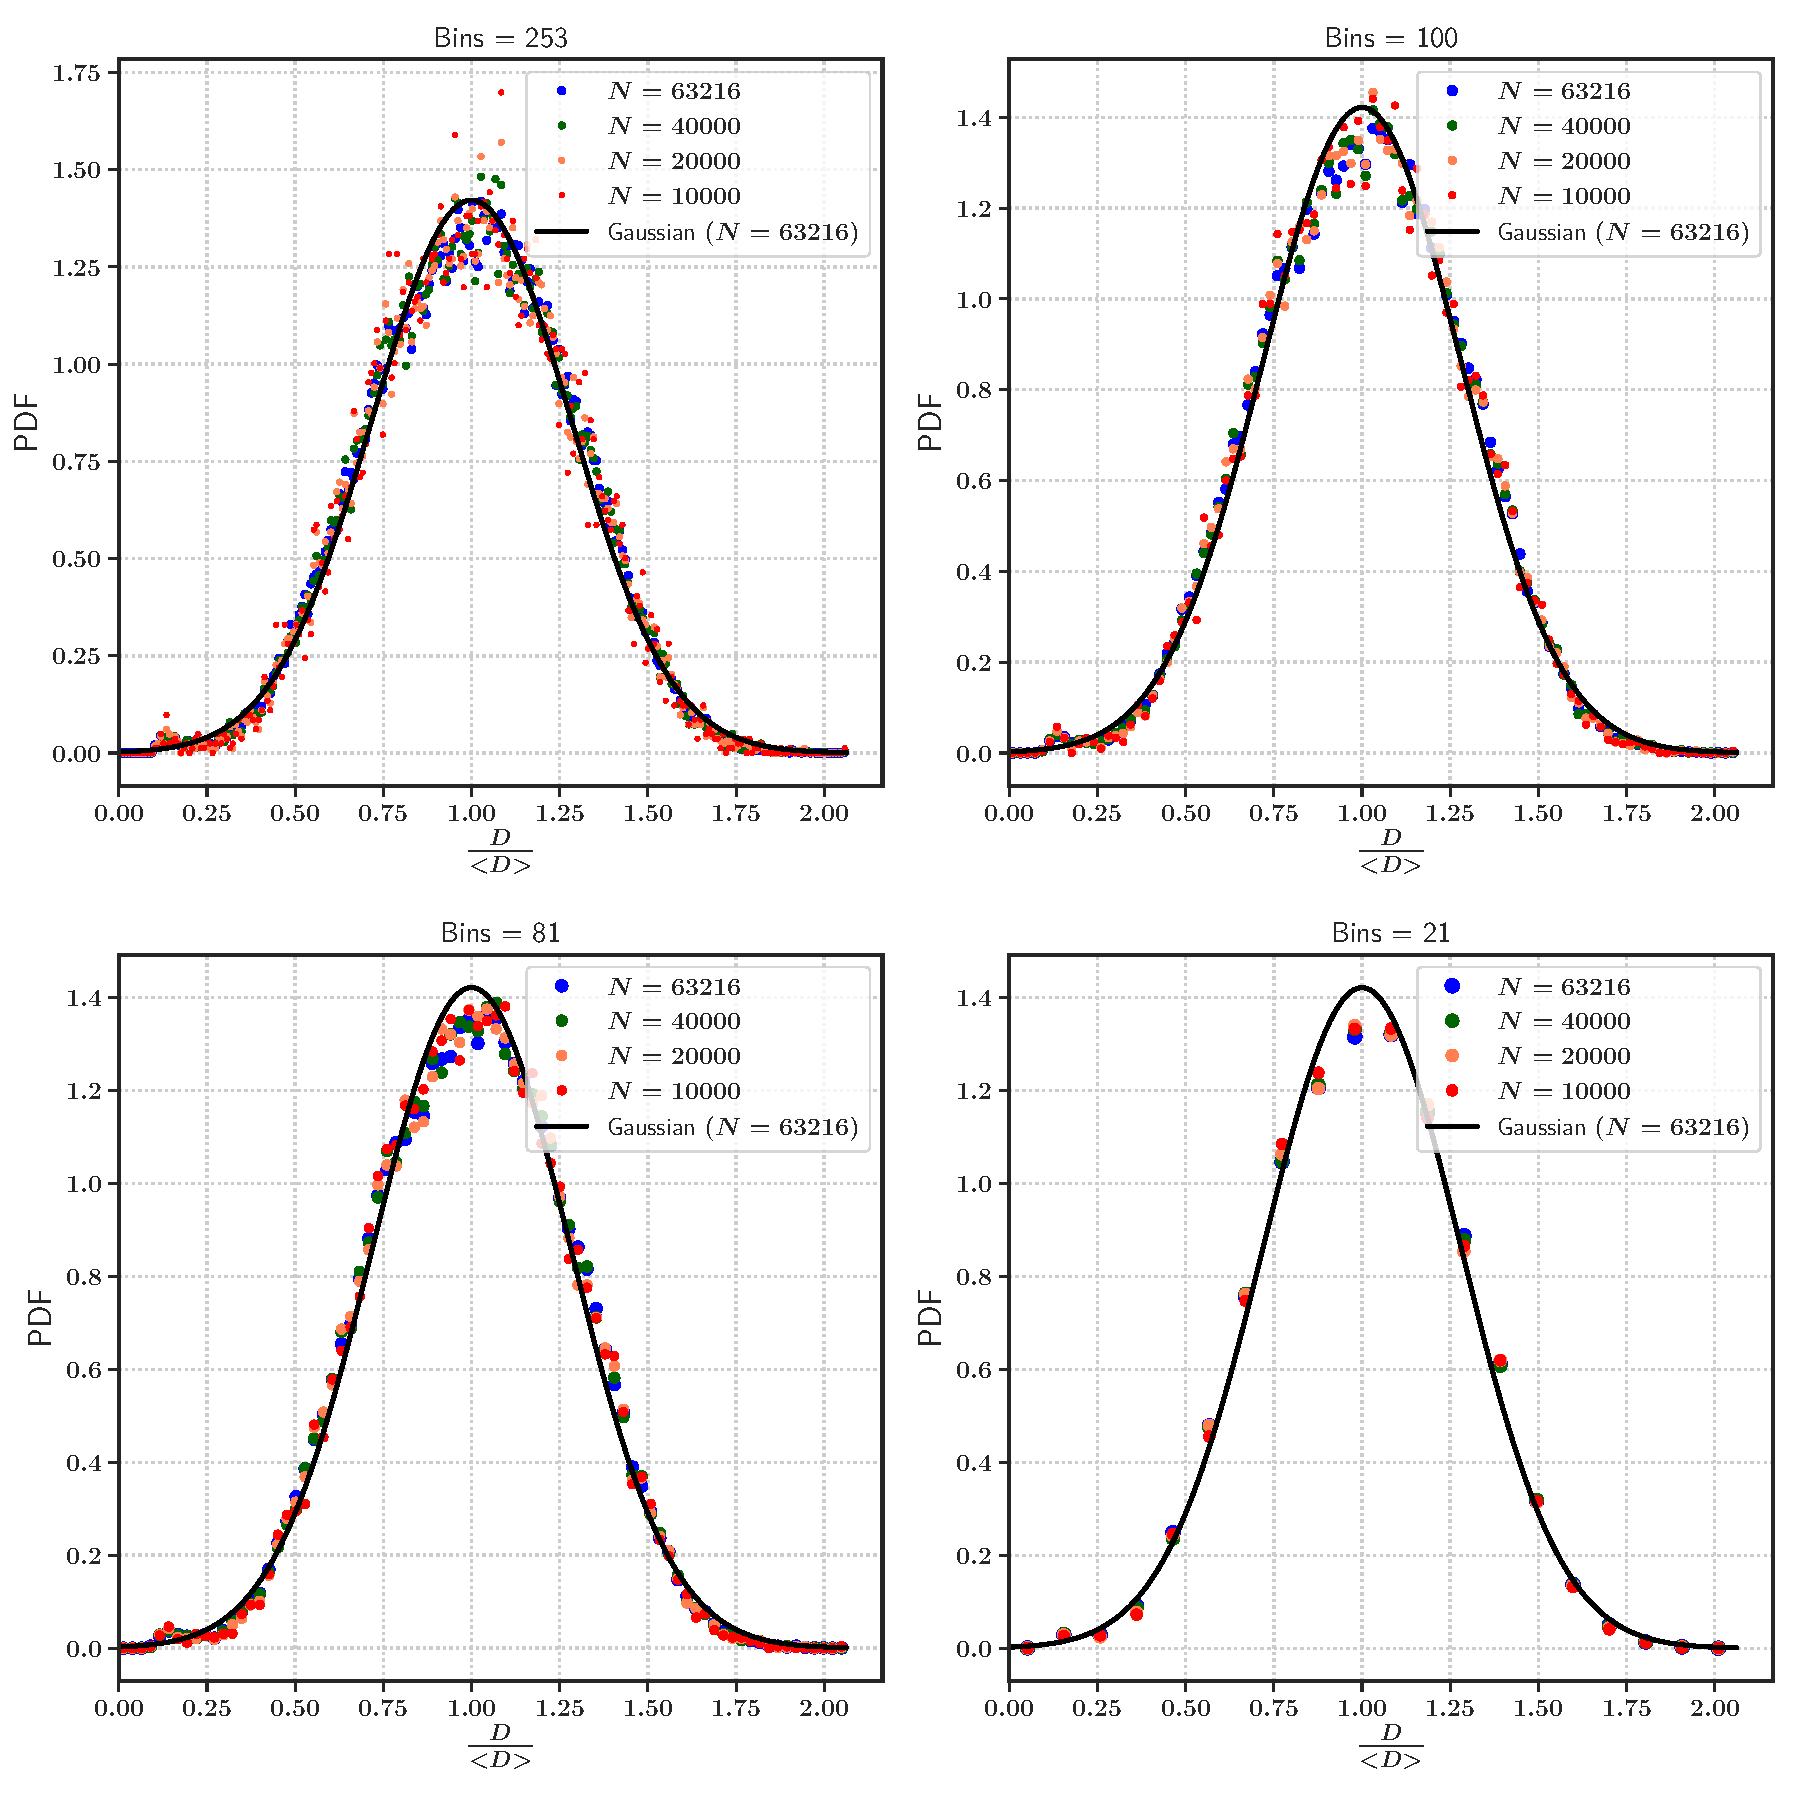
\includegraphics{plots/drop_stats/long_time_diameter_bins.pdf}
\caption{Probability distribution functions of the droplet diameter at time $T = 30$. 
The ensemble is characterized by $\Phi_0 \equiv \left( Oh = 10^{-2}, K = 2\pi , \varepsilon = 1.0 , \Lambda = 50 \right)$. 
The diameters are normalized by the mean of the corresponding sample.  
The distributions are generated using datasets corresponding to four different sample sizes, 
including four different choices of (uniform) bin width. 
The Gaussian functions are characterized by the mean and variance of the original dataset, 
hence they are plotted alongside the histograms instead of being fitted to the bin heights.
	}
\label{t2_dia_bins}
\end{figure*}

% PDF predictions of data at long times


\begin{figure*}
\centering
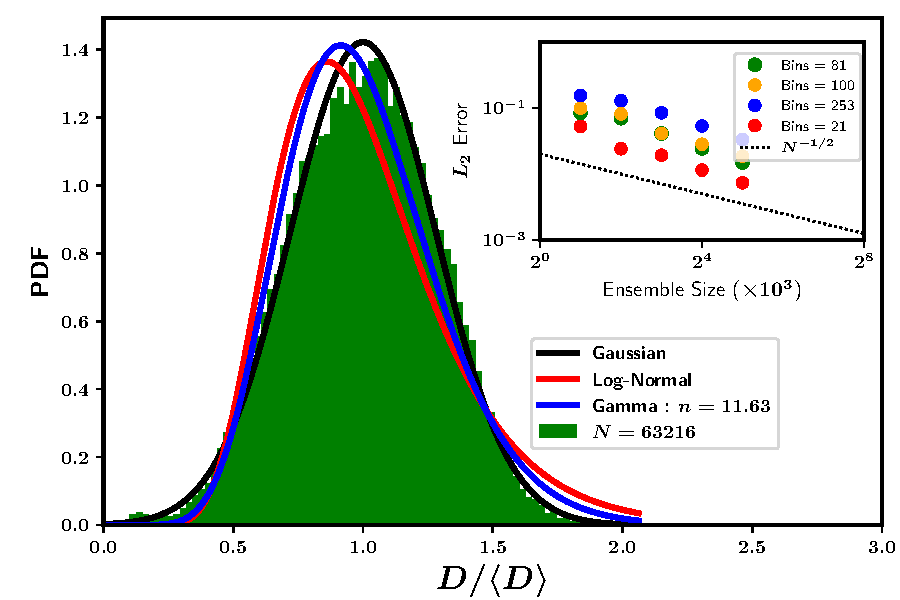
\includegraphics{plots/drop_stats/long_time_diameter_fits.pdf}
\caption{Probability distribution functions of the droplet diameter at time $T = 30$. 
The ensemble is characterized by $\Phi_0 \equiv \left( Oh = 10^{-2}, K = 2\pi , \varepsilon = 1.0 , \Lambda = 50 \right)$. 
The diameters are normalized by the mean of the corresponding sample.  
The distribution is generated using 81 bins of uniform size, represented in green.  
The Gaussian and Log-Normal functions are characterized by the mean and variance of the original dataset, 
therefore are plotted alongside the histogram, whereas, the Gamma function is fitted to the bin heights,
with $n= 11.63$ being the value corresponding to the best fit.
	}
\label{t2_dia_fits}
\end{figure*}

% N^{-1/2} scaling of error 

In Fig. \ref{t2_dia_fits}, we present a comparison of the different probaility 
density functions applied to the largest ensemble of drops characterized by $\Phi_0$ and $T=30$. 
The Gaussian is found to be the best approximation to the normalized 
diameter distribution, followed by the Gamma and Log-Normal functions.
The Gaussian and Log-Normal curves are generated using the mean and variance 
of the dataset, whereas the free parameter $n$ of the Gamma function is determined
according to the best least-squares fit over the histogram. 
A noteworthy point demonstrated by the inset of Fig. \ref{t2_dia_fits} is that
the error \sidenote{The error is defined as the $L_2$ norm of the differences 
between the bin hights of the sample and the largest sample, where both 
samples have identical bin-width.} scales as $N^{-1/2}$, $N$ being the sample size.
Additionally, the scaling is not sensitive to the choice of bin-width. 
This strongly suggests the absence of any unforeseen correlations between the 
individual realizations (corrugated ligaments) that form the ensemble.


\subsection*{Volume Distributions}

We now shift our attention towards the distribution of droplet volumes. 
Figures \ref{t1_vol_bins} and \ref{t2_vol_bins} show the PDFs 
of the normalized droplet volume corresponding to $T=15$ and $T=30$ respectively. 
The volumes are normalized by the means of the associated samples. 
As in the diameter distributions, the bin widths are always 
based on the properties of the largest sample.
In stark contrast to the case of the diameters, the drop volumes
are found to be heavily skewed towards the smaller sizes.
Similar to the diameter PDFs, the choice of bin-width seems to not have any considerable impact
on the overall shape of the distribution, and is also independent of the sample size.   
In this case though, the single parameter Gamma density function \eqref{gamma} appears to
be the approximation to the volume distribution, with the best fit corresponding to 
values of $n \approx 1.68$ and $n \approx 1.58$ corresponding to $T=15$ and $T=30$ respectively.
There is a slight dependence of the parameter $n$ on the bin-width, which is expected 
as $n$ itself is determined according to the best fit to the histogram in question.

% short time scale 

\begin{figure*}
\centering
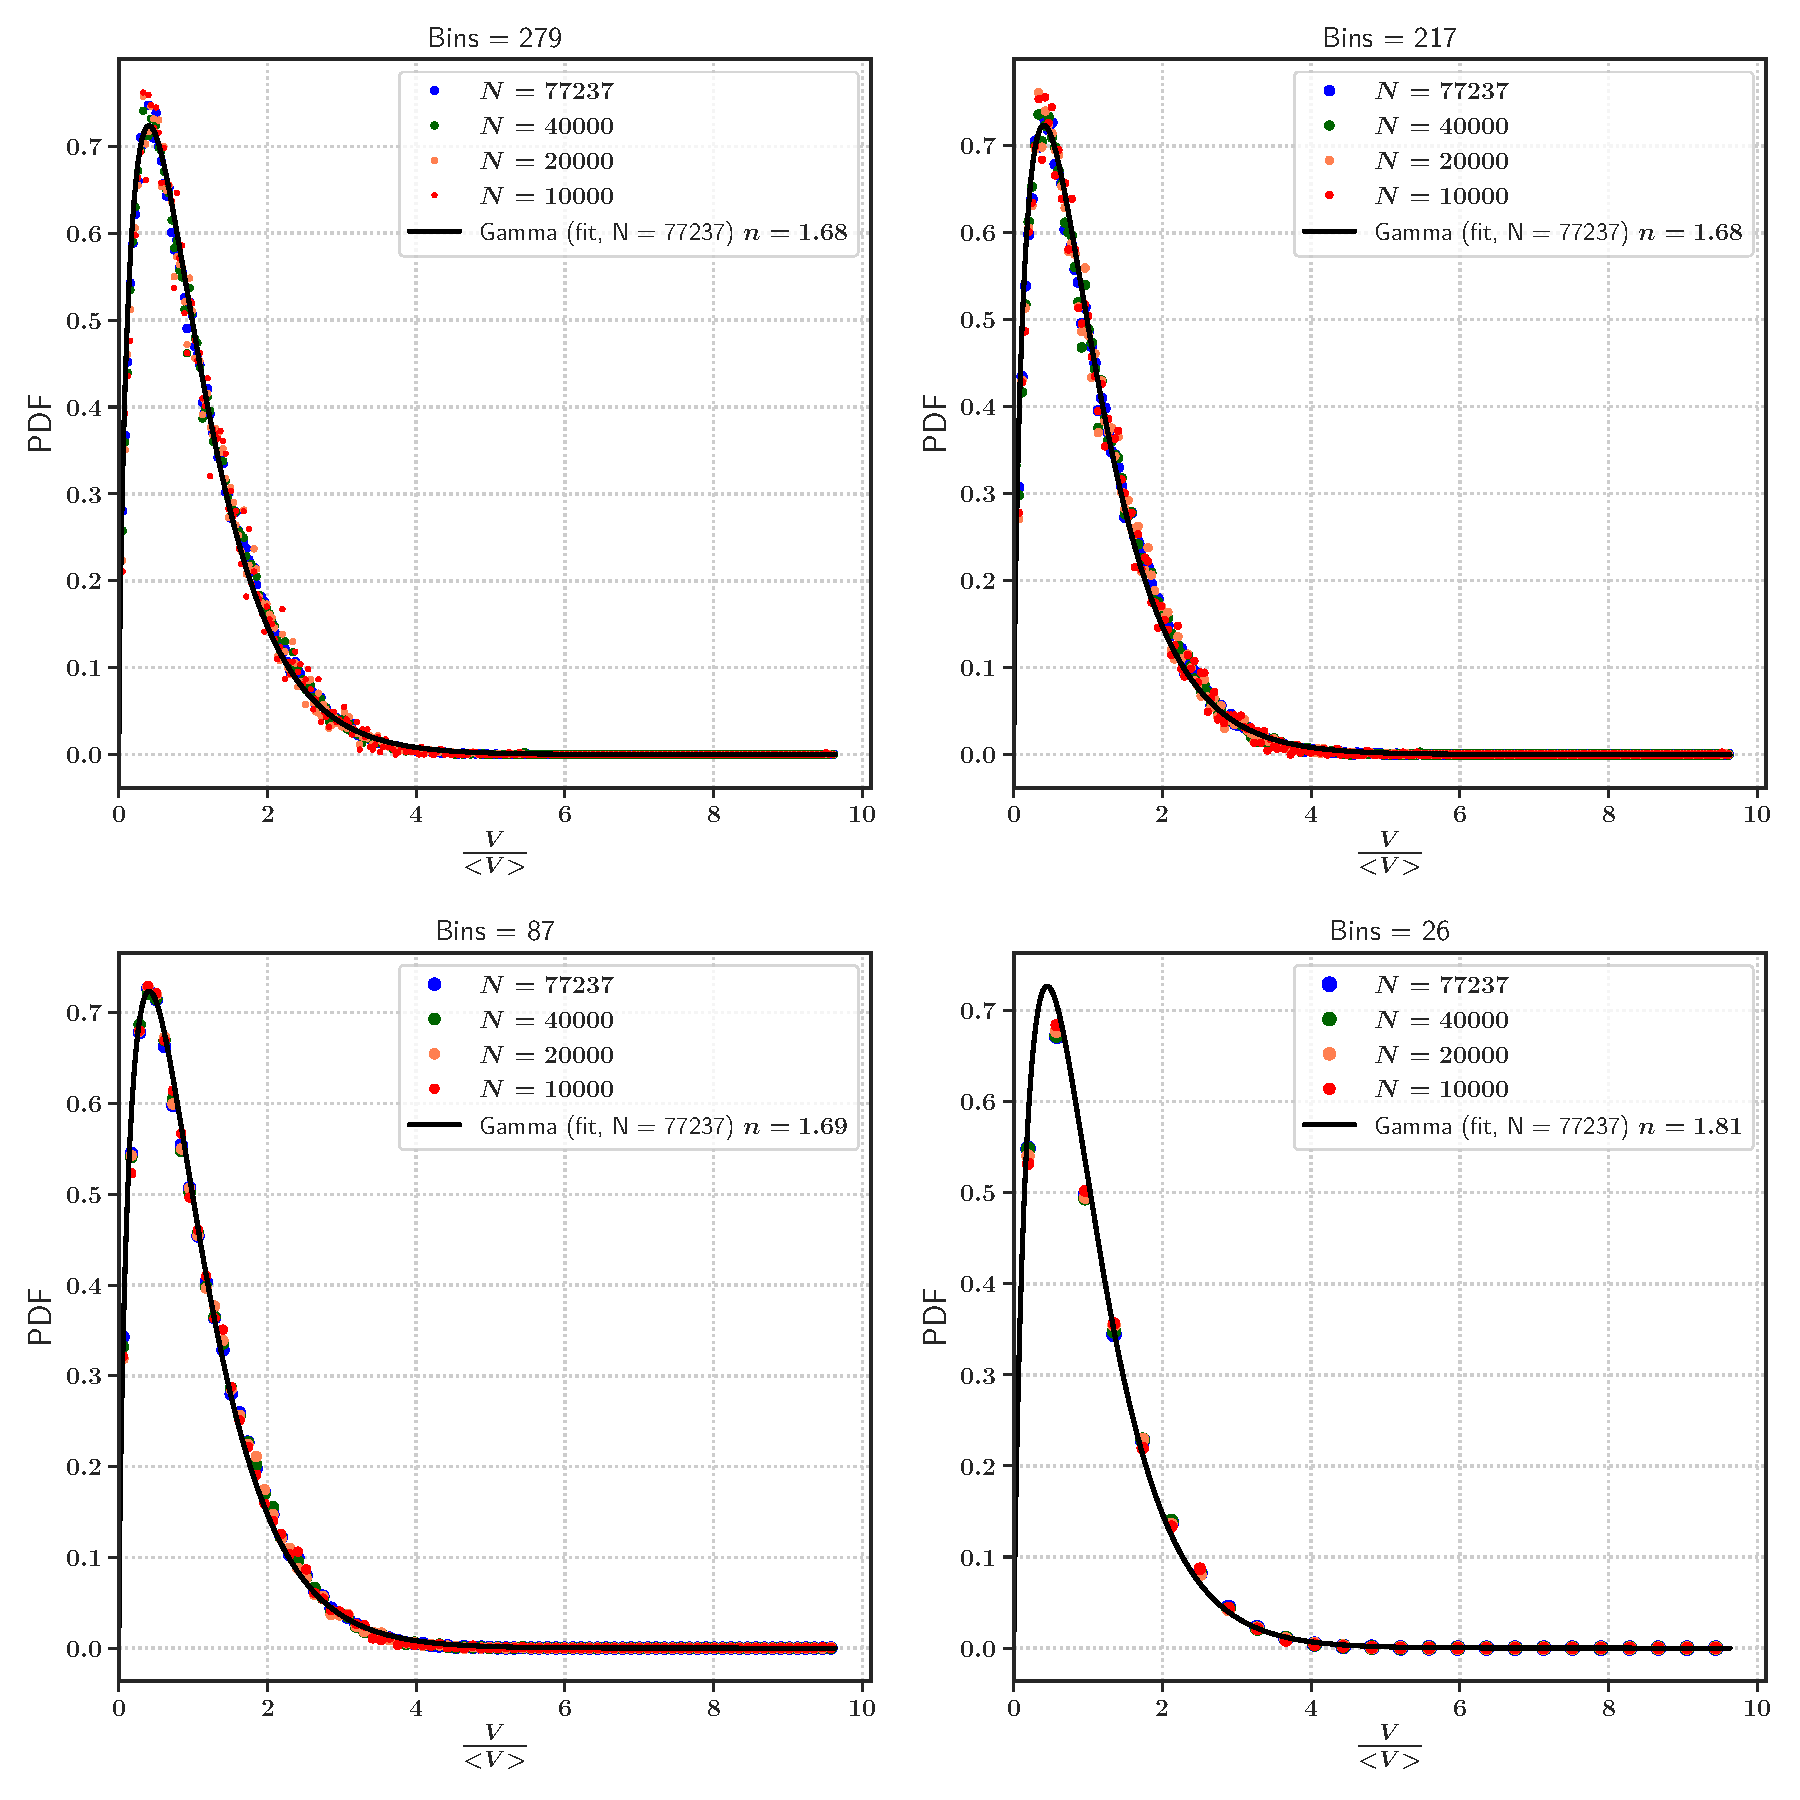
\includegraphics{plots/drop_stats/short_time_volume_bins.pdf}
\caption{Probability distribution functions of the droplet volume at time $T = 15$. 
The ensemble is characterized by $\Phi_0 \equiv \left( Oh = 10^{-2}, K = 2\pi , \varepsilon = 1.0 , \Lambda = 50 \right)$. 
The volumes are normalized by the mean of the corresponding sample.  
The distributions are generated using datasets corresponding to four different sample sizes, 
including four different choices of (uniform) bin width. 
The Gamma functions are characterized by the parameter $n$, the value of which is determined 
by that which provides the best (least-squares) fit to the corresponding bin heights.  
	}
\label{t1_vol_bins}
\end{figure*}

% long time scale

\begin{figure*}
\centering
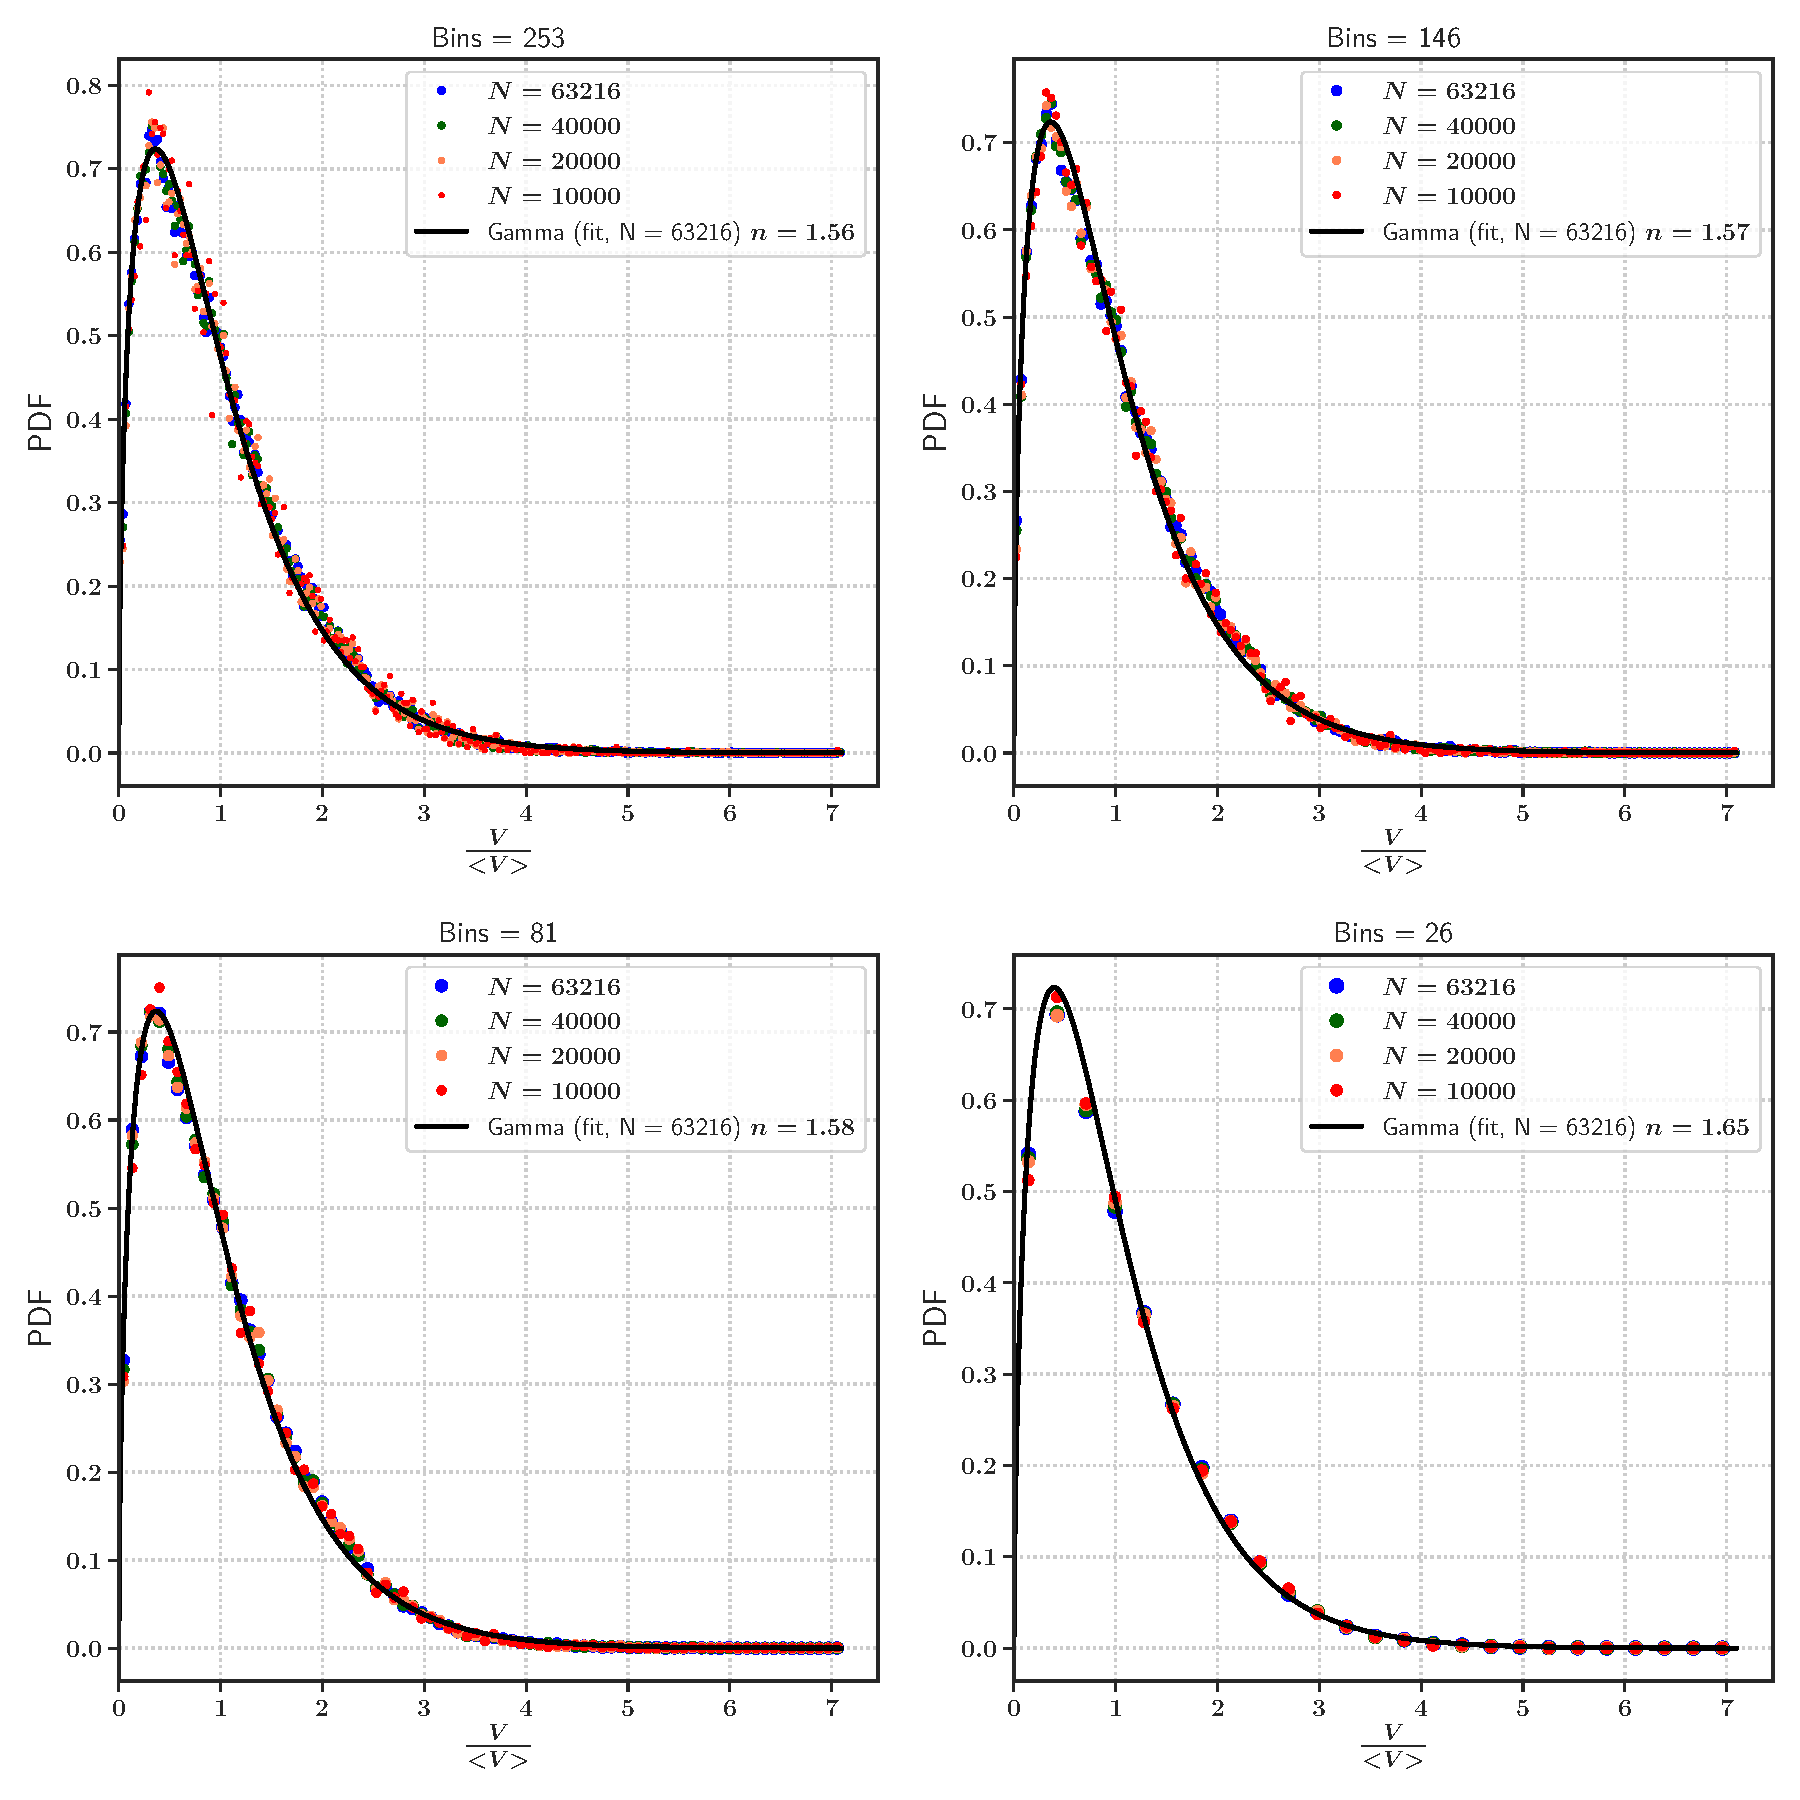
\includegraphics{plots/drop_stats/long_time_volume_bins.pdf}
\caption{Probability distribution functions of the droplet volume at time $T = 30$. 
The ensemble is characterized by $\Phi_0 \equiv \left( Oh = 10^{-2}, K = 2\pi , \varepsilon = 1.0 , \Lambda = 50 \right)$. 
The volumes are normalized by the mean of the corresponding sample.  
The distributions are generated using datasets corresponding to four different sample sizes, 
including four different choices of (uniform) bin width. 
The Gamma functions are characterized by the parameter $n$, the value of which is determined 
by that which provides the best (least-squares) fit to the corresponding bin heights.  
	}
\label{t2_vol_bins}
\end{figure*}

Fig. \ref{t2_vol_fits} shows a comparison of the different probaility 
density functions applied to the largest ensemble of drops characterized by $\Phi_0$ and $T=30$. 
The Gamma density function is found to be the best approximation to the normalized 
volume distribution, followed by the Log-Normal and Gaussian functions.
Similar to the diameter case, the Gaussian and Log-Normal curves are 
generated using the mean and variance of the dataset, 
whereas the free parameter $n$ of the Gamma function is determined
according to the best least-squares fit over the histogram. 
As seen before, the error (inset of Fig. \ref{t2_vol_fits}) 
scales as $N^{-1/2}$, regardless of the binning criteria used. 

% PDF predictions of data at long times

\begin{figure*}
\centering
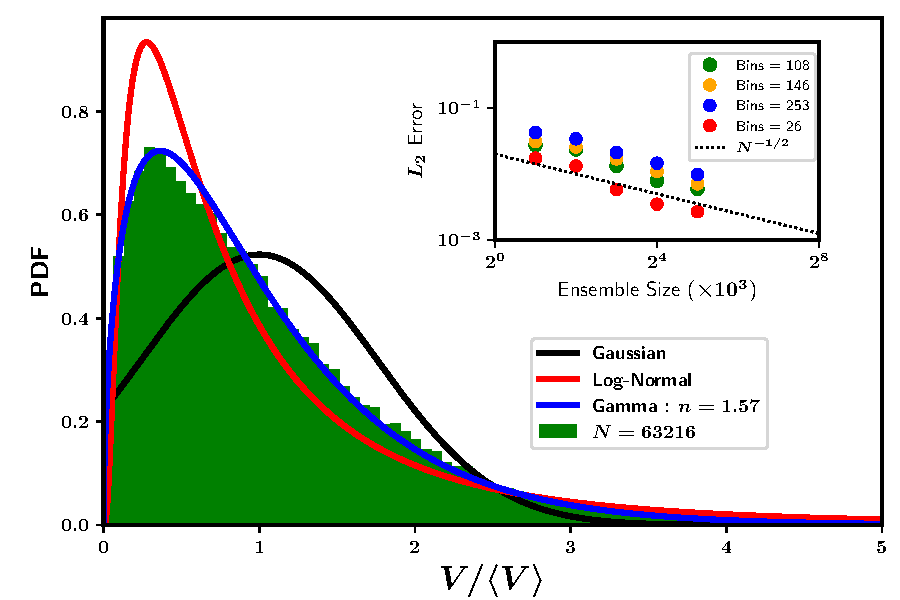
\includegraphics{plots/drop_stats/long_time_volume_fits.pdf}
\caption{Probability distribution functions of the droplet volume at time $T = 30$. 
The ensemble is characterized by $\Phi_0 \equiv \left( Oh = 10^{-2}, K = 2\pi , \varepsilon = 1.0 , \Lambda = 50 \right)$. 
The diameters are normalized by the mean of the corresponding sample.  
The distribution is generated using 108 bins of uniform size, represented in green.  
The Gaussian and Log-Normal functions are characterized by the mean and variance of the original dataset, 
therefore are plotted alongside the histogram, whereas, the Gamma function is fitted to the bin heights,
with $n= 1.57$ being the value corresponding to the best fit.
	}
\label{t2_vol_fits}
\end{figure*}

% N^{-1/2} scaling of error 


\subsection*{Influence of Corrugation Amplitude}

\begin{marginfigure}[2cm]
\centering
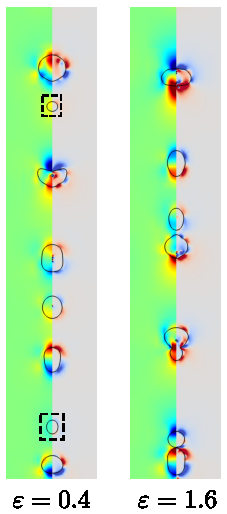
\includegraphics{plots/drop_stats/amp_long_compare.pdf}
	\caption{The fate of two ligaments whose initial surfaces 
	are created using the same set of random overlapping waves, 
	but differ by the strength of the perturbations.
	The ligament on the left is part of ensemble $\Phi_1$ 
	and the one on the right is part of $\Phi_2$. 
	The droplets enclosed in the boxes (dashed lines)
	are characteristic of the distintegration of weakly perturbed ligaments,
	wherein their sizes are smaller than the typical size at least by a factor of $2$. 
	}
\label{amp_long_comp}
\end{marginfigure}

As discussed in the previous chapter, the ``smoothness'' of the initial geometrical
shape of the ligament is expected to have a significant influence on the 
destabilization of the liquid thread and the concomitant coalescence dynamics.
In order to ascertain the impact of the strength of the initial perturbations
on the resulting drop size distribution, we conduct simulations of two different 
millimeter scale ensembles $\Phi_1$ and $\Phi_2$. Both of them are characterized 
by the same set of adimensional parameters as in $\Phi_0$, except that $\varepsilon = 0.4$
in case of $\Phi_1$, whereas $\varepsilon = 1.6$ in case of $\Phi_2$.

For the case of weakly perturbed ligaments, Fig. \ref{tseries_small} 
demonstrates the temporal evolution of the droplet diameter distributions, 
where the diameter is rescaled by the (mean) width $W$ of the initial ligaments. 
At small time scales, the distribution is bimodal in nature, consisting of a large
number of drops that are quite smaller than even the initial ligament width. 
This may be a consequence of the non-linear effects \cite{satellite_1,satellite_2} 
that kick in immediately following the initial linear (exponential) growth phase, 
often resulting in the liquid thread disintegrating into a collection of main 
and (significantly smaller) satellite drops (see Fig. \ref{amp_comp} in the preceding chapter). 
At large times, the peak corresponding to the smaller sizes is considerably diminished, 
whereas the larger size peak develops into more of a ``plateau'' type shape.  
This observed shifts in the distribution as a function of time can be explained by the 
successive coalescences taking place, where the smallest drops coalesce with the largest drops.
By largest drops, we mean the ones situated to the right of the large size peak, 
corresponding to the region of the distribution which eventually gives rise to the plateau shape.


Coming to the strongly perturbed ligament shapes, Fig. \ref{tseries_large} illustrates 
the unimodal character of the overall distribution shape.
There seems to be a lack of any significant qualitative change 
when comparing the distributions at small and large time scales. 
The large amplitude perturbations of the ligament surface do not 
allow for any significant amount of liquid rearrangement within the bulk prior 
to disintegration, thus the collection of drops formed immediately following the breakup
of the thread-like structure are quite disperse when with respect to their sizes.
The mean of the distribution displays a slight shift towards the larger sizes, with the passage of time. 
This shift can be explained by the effect of random coalescences amongst droplets corresponding to all sizes.

To summarize, in Fig. \ref{tseries_comp} we present a side-by-side comparison of 
the aforementioned temporal evolutions of the droplet diameter distributions.  
We infer that the primary influence of the corrugation strength 
is that it changes the nature of the resulting distribution from bimodal to unimodal,
as one increases the amplitude of the initial perturbations. 
Although the dynamics of the droplet coalescences (post-breakup) follow different trajectories
in accordance with the corrugation strength (see Fig. \ref{amp_long_comp}), 
the distributions at large times end up looking rather similar.

% temporal variation in drop size PDF's for low and high levels of corrugation

\begin{figure}
\centering
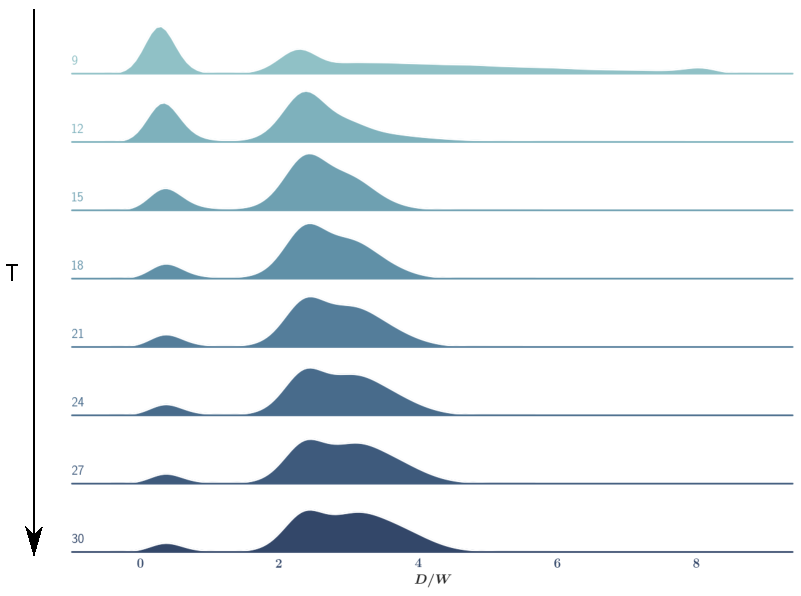
\includegraphics{plots/drop_stats/small_amp.pdf}
\caption{Temporal evolution of the probability distribution functions of the droplet diameter.
	The diameter is rescaled by the initial width $W$ of the ligaments.
	The ensemble is characterized by $\Phi_1 \equiv \left( Oh = 10^{-2}, K = 2\pi 
, \varepsilon = 0.4 , \Lambda = 50 \right)$, thus consisting of \textit{weakly} perturbed 
initial ligaments shapes. 
	}
\label{tseries_small}
\end{figure}

\begin{figure}
\centering
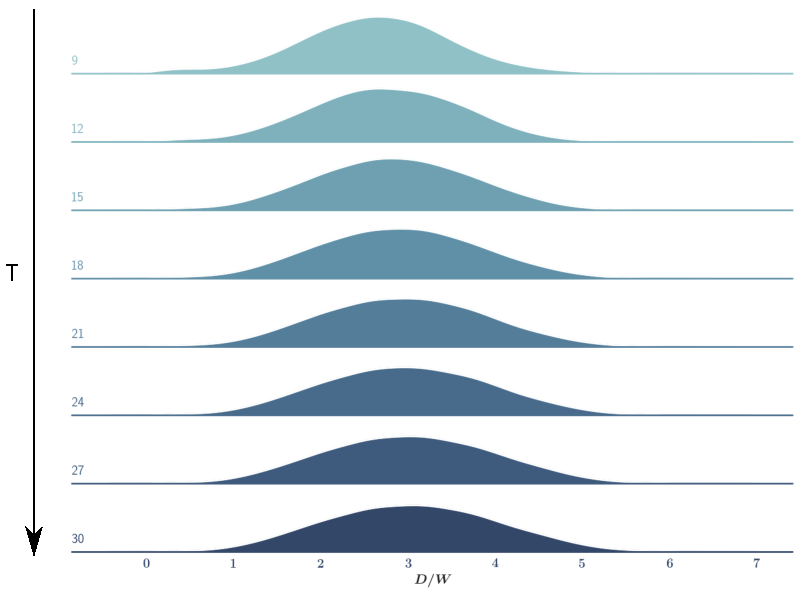
\includegraphics{plots/drop_stats/large_amp.pdf}
\caption{Temporal evolution of the probability distribution functions of the droplet diameter.
	The diameter is rescaled by the initial width $W$ of the ligaments.
	The ensemble is characterized by $\Phi_2 \equiv \left( Oh = 10^{-2}, K = 2\pi 
, \varepsilon = 1.6 , \Lambda = 50 \right)$, thus consisting of \textit{strongly} perturbed 
initial ligaments shapes. 
	}
\label{tseries_large}
\end{figure}

% side by side comparison
% extrapolations of RP etc , limit of volume of largest drop


\begin{figure*}
\centering
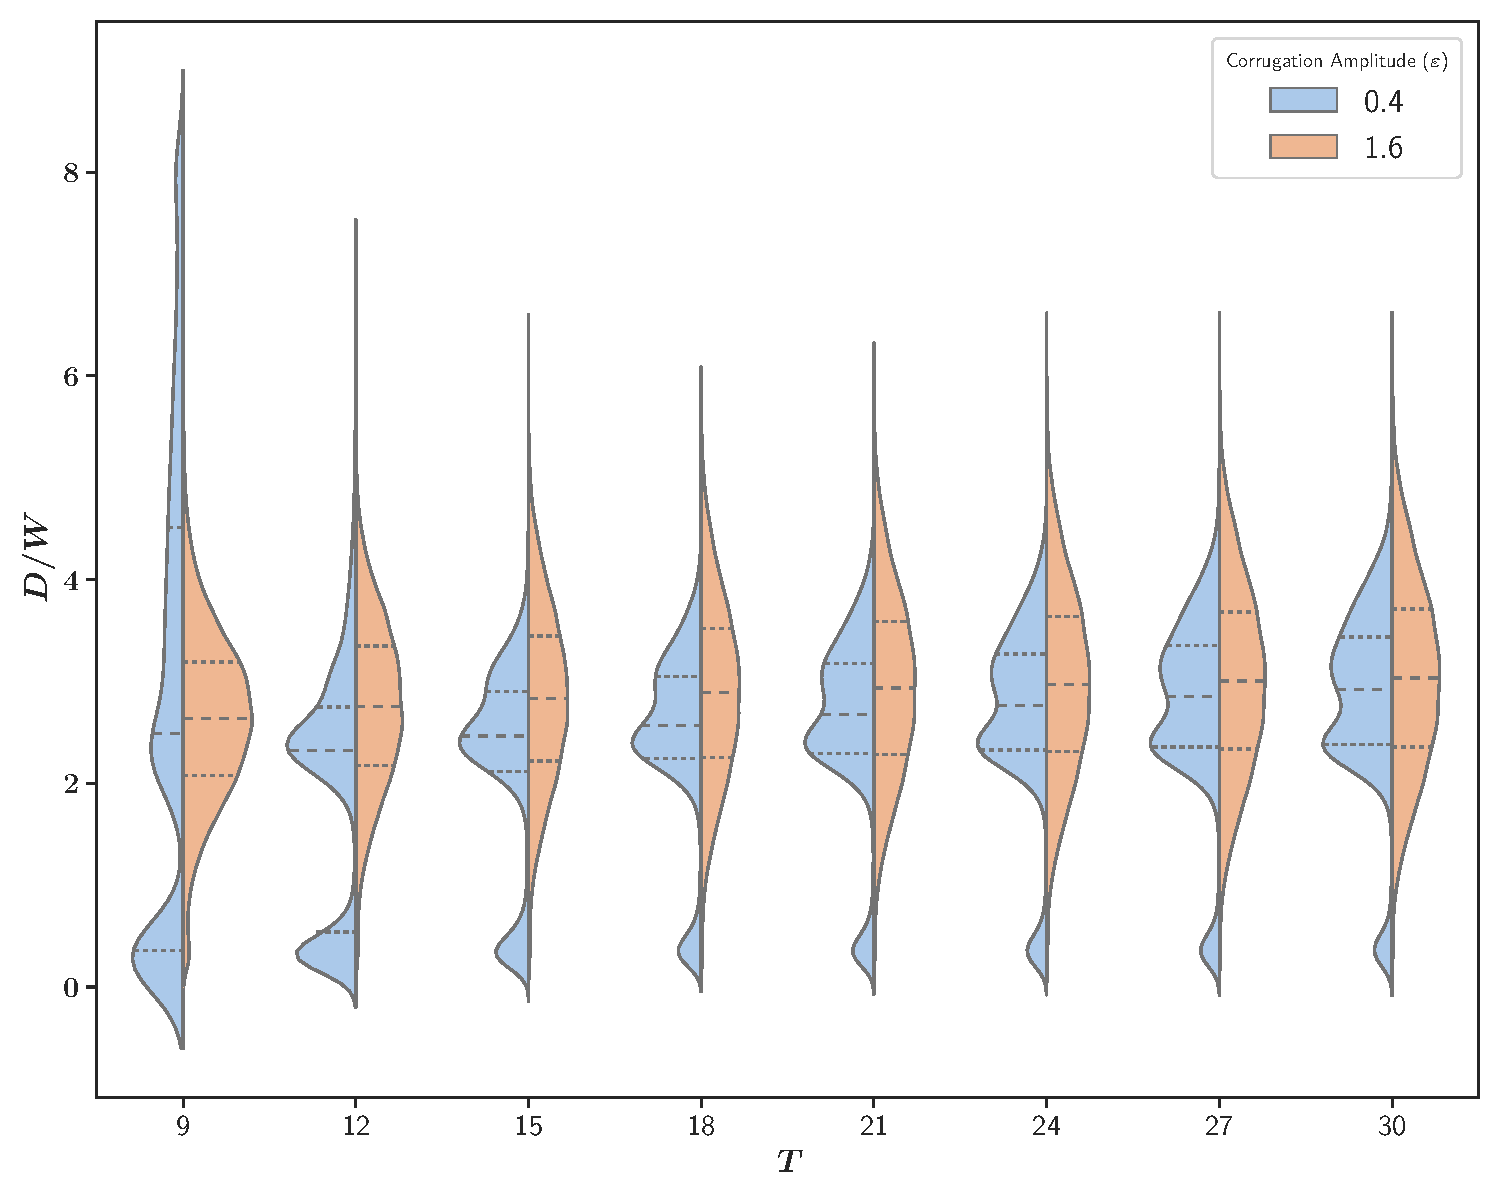
\includegraphics{plots/drop_stats/amp_dist_compare.pdf}
\caption{Comparison between the temporal evolution of the probability distribution functions of the
	droplet diameter, corresponding to the strongly ($\varepsilon = 0.4$) and 
	weakly ($\varepsilon = 1.6$) perturbed ligament ensembles. 
	The diameter is rescaled by the width of the initial ligament. 
	The ensembles are characterized by $\Phi_{\{1,2\}} \equiv \left( Oh = 10^{-2}, K = 2\pi 
, \varepsilon = \{0.4,1.6 \} , \Lambda = 50 \right)$. 
The thick dashed lines correspond to the mean of the respective distribution, and the thinner
dashed lines located on both sides of the thicker line corresponding to the respective interquartile ranges. 
	}
\label{tseries_comp}
\end{figure*}


\section{Description of Large Sizes}


% estimation of error with binomial distribution



% linear fitting, with and without uncertainty, full distribution and tail zoom  

% methodology to determine best fit

\begin{figure}
\centering
	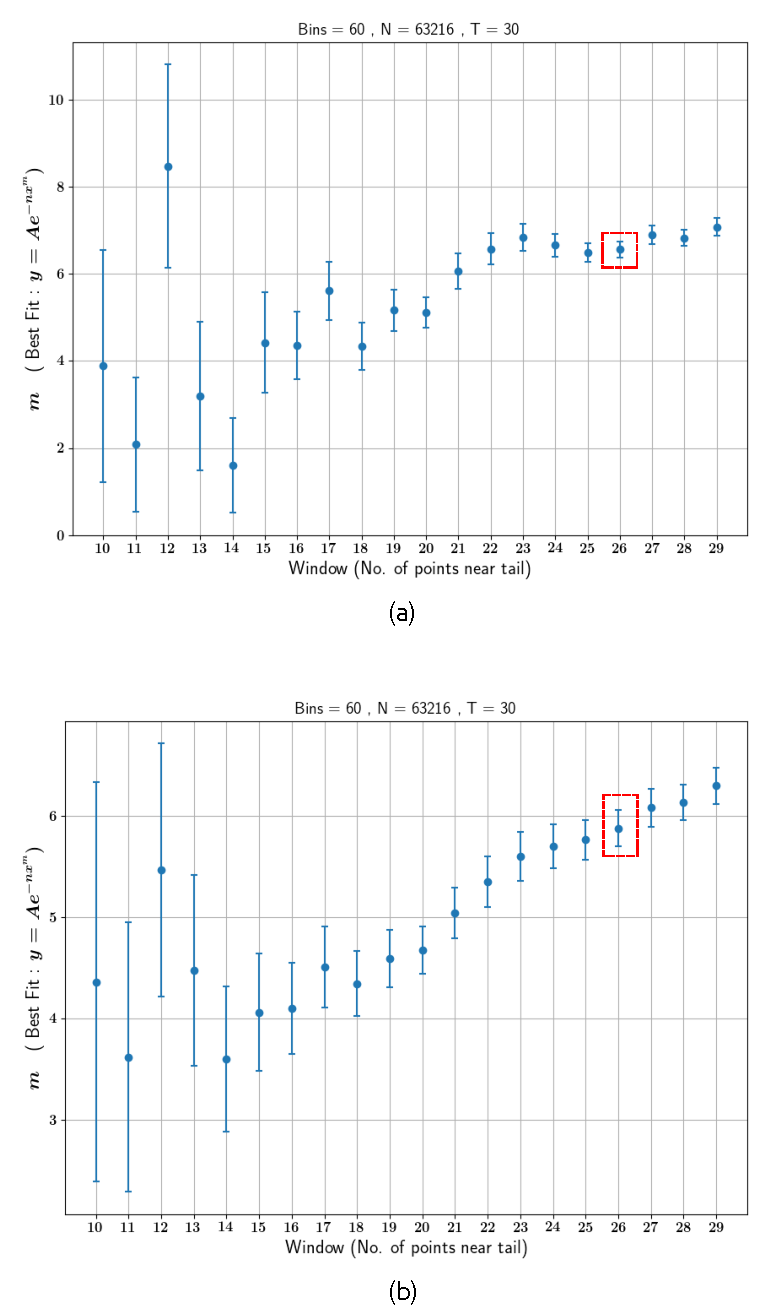
\includegraphics{plots/drop_stats/determine_fit_linear.pdf}
	\caption{\blindtext}
\label{determine_linear}
\end{figure}


% without uncertainty

\begin{figure}
\centering
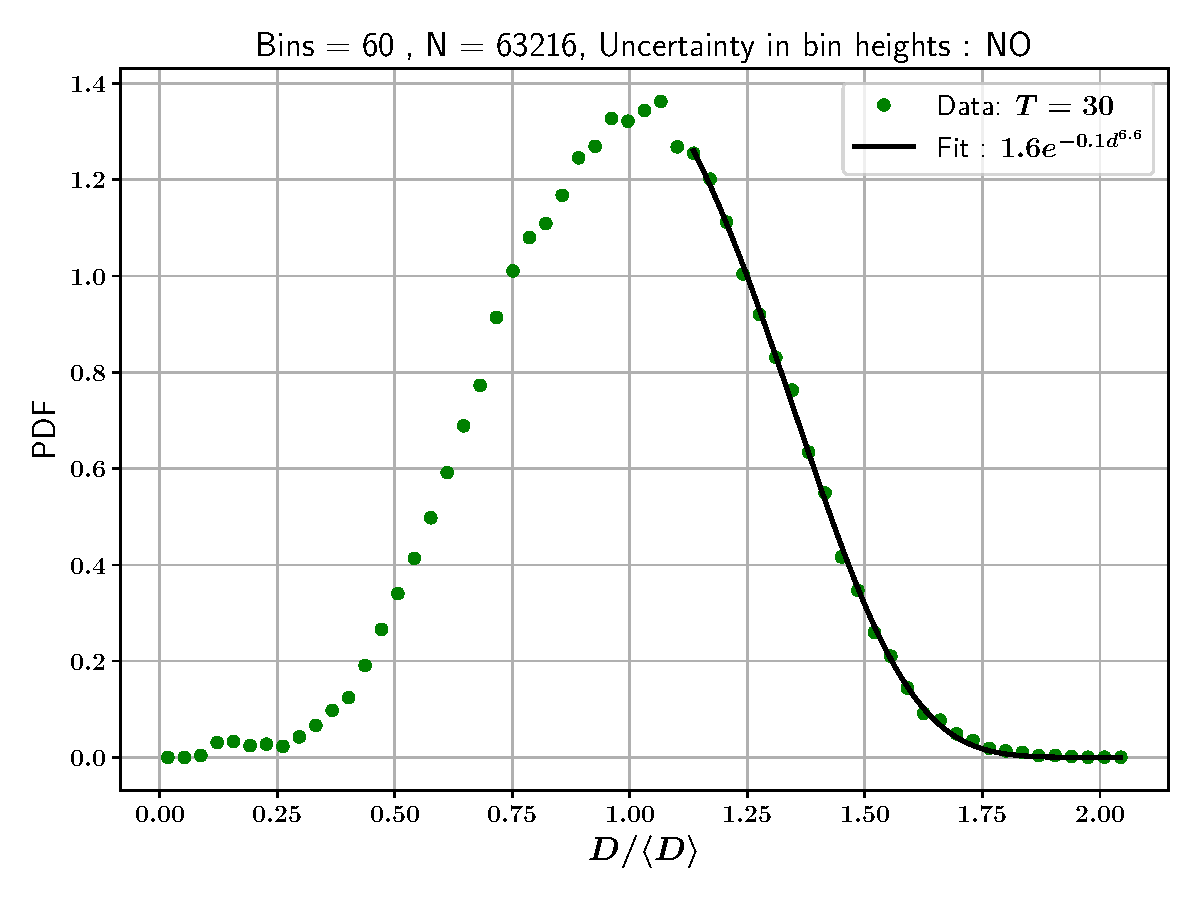
\includegraphics{plots/drop_stats/linear_tail_fit_uncertainty_no.pdf} \\
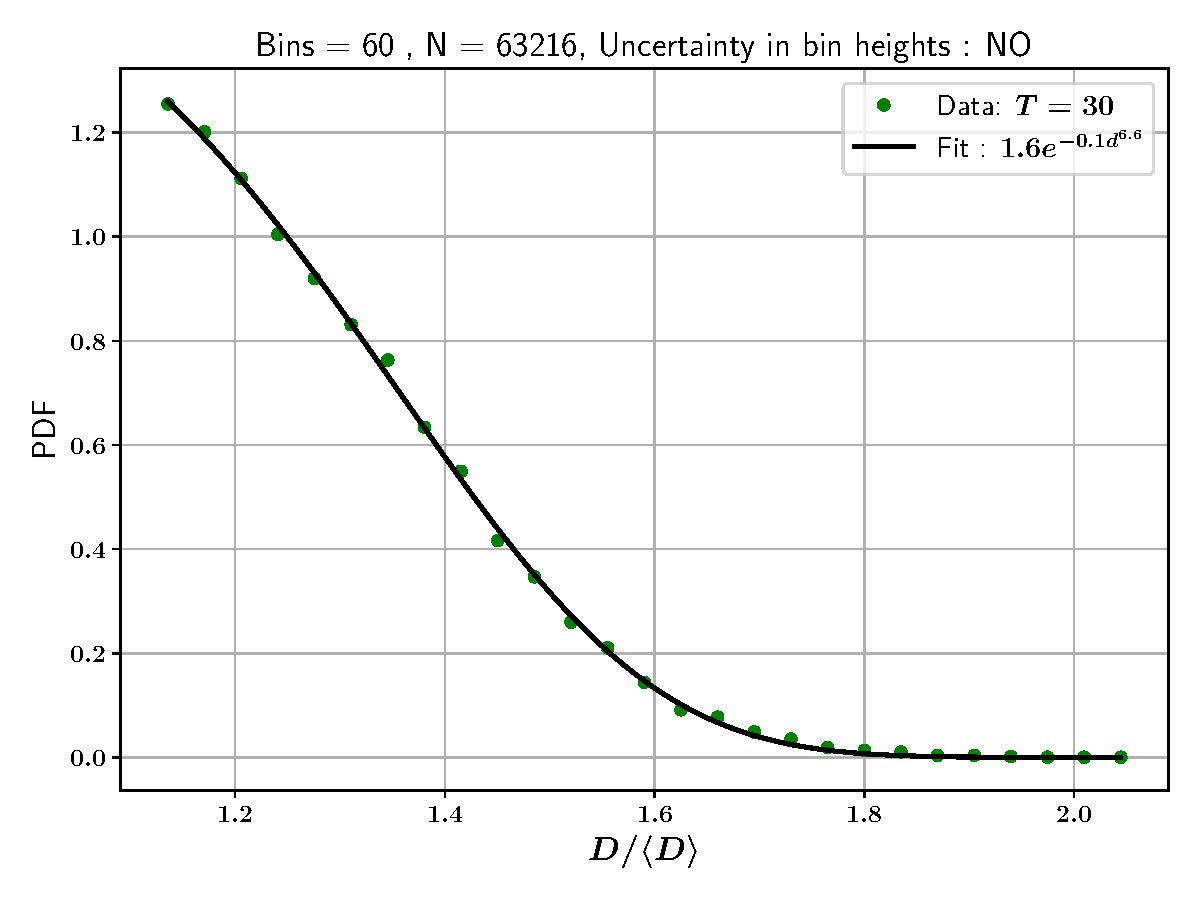
\includegraphics{plots/drop_stats/linear_zoom_tail_fit_uncertainty_no.pdf} \\ 
\caption{\blindtext}
\label{linear_fits_wo}
\end{figure}

% with uncertainty

\begin{figure}
\centering
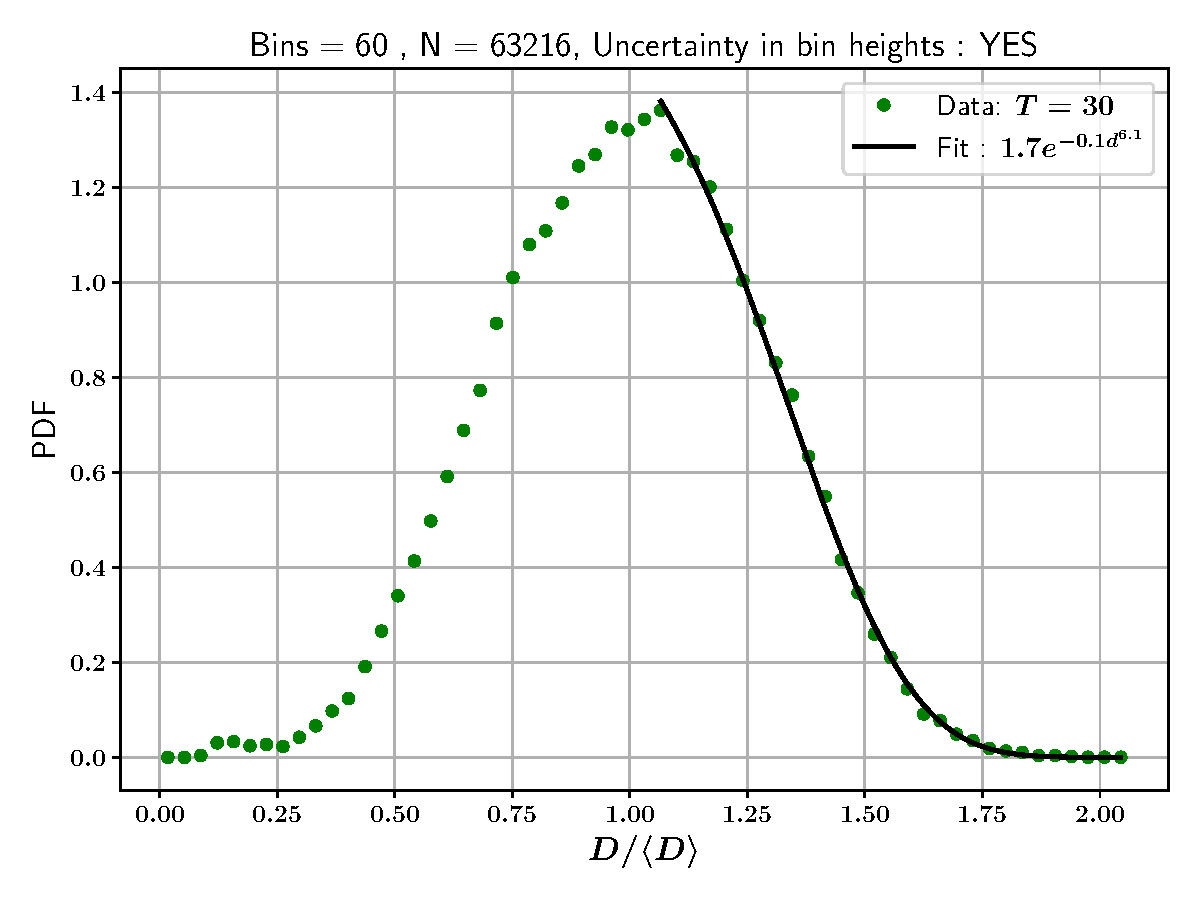
\includegraphics{plots/drop_stats/linear_tail_fit_uncertainty_yes.pdf} \\
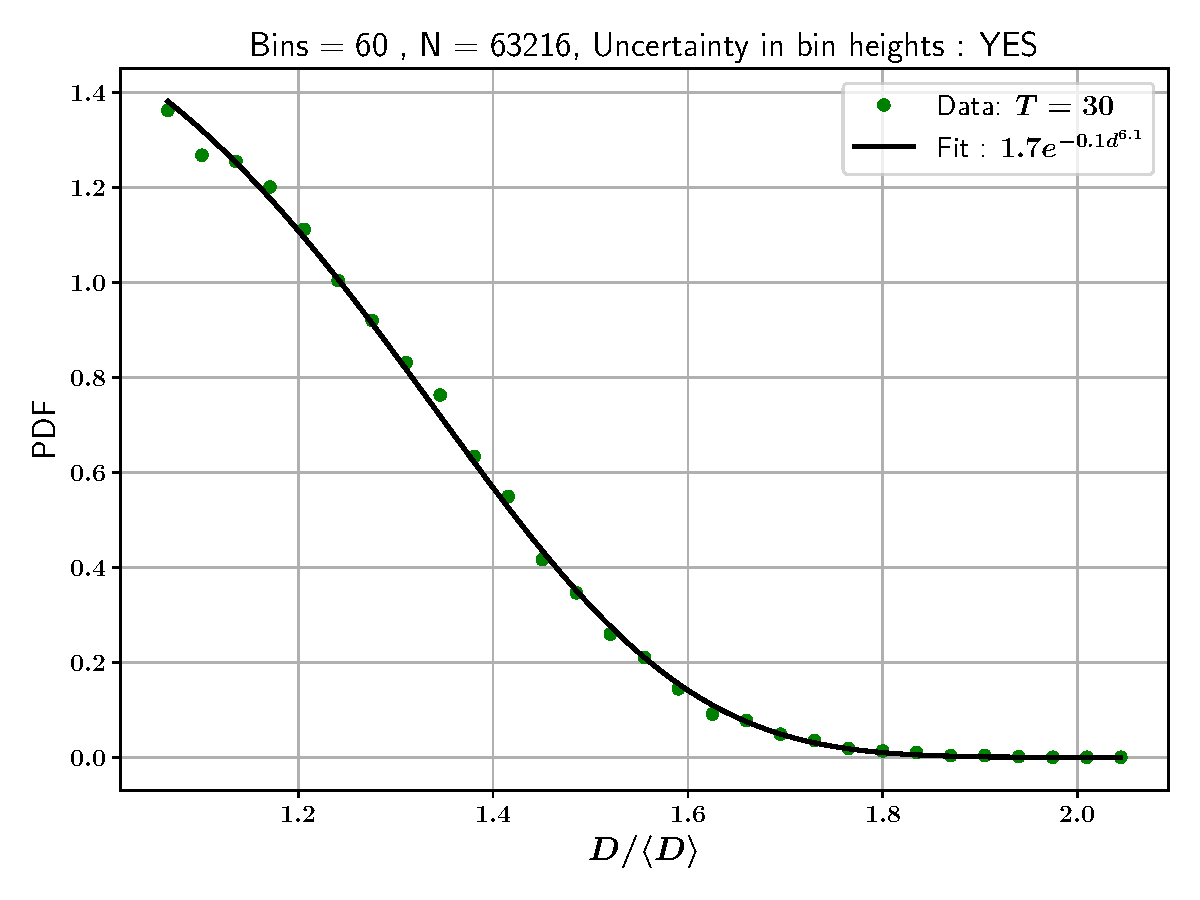
\includegraphics{plots/drop_stats/linear_zoom_tail_fit_uncertainty_yes.pdf} \\ 
\caption{\blindtext}
\label{linear_fits_with}
\end{figure}


% log(log) vs log fitting, with and without uncertainty, full distribution and tail zoom  

% methodology to determine best fit

\begin{figure}
\centering
	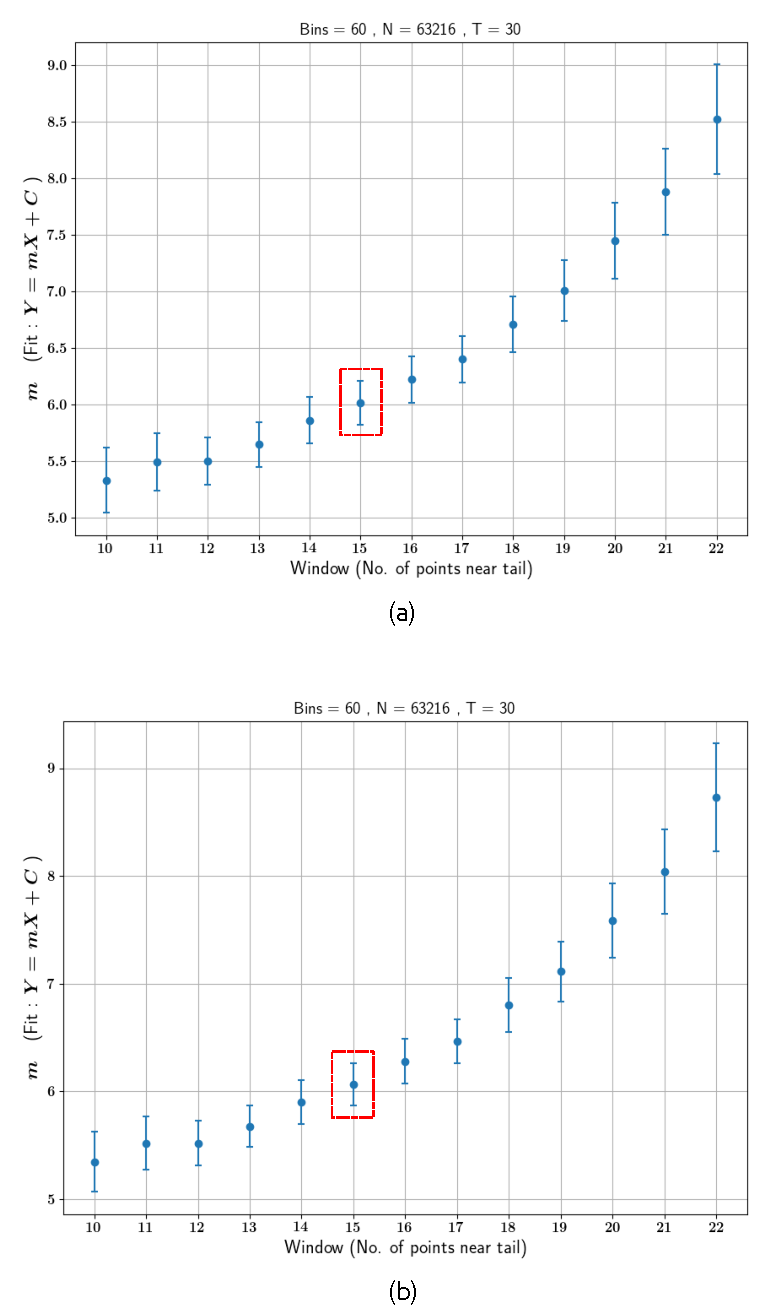
\includegraphics{plots/drop_stats/determine_fit_log.pdf}
	\caption{\blindtext}
\label{determine_log}
\end{figure}

% without uncertainty

\begin{figure}
\centering
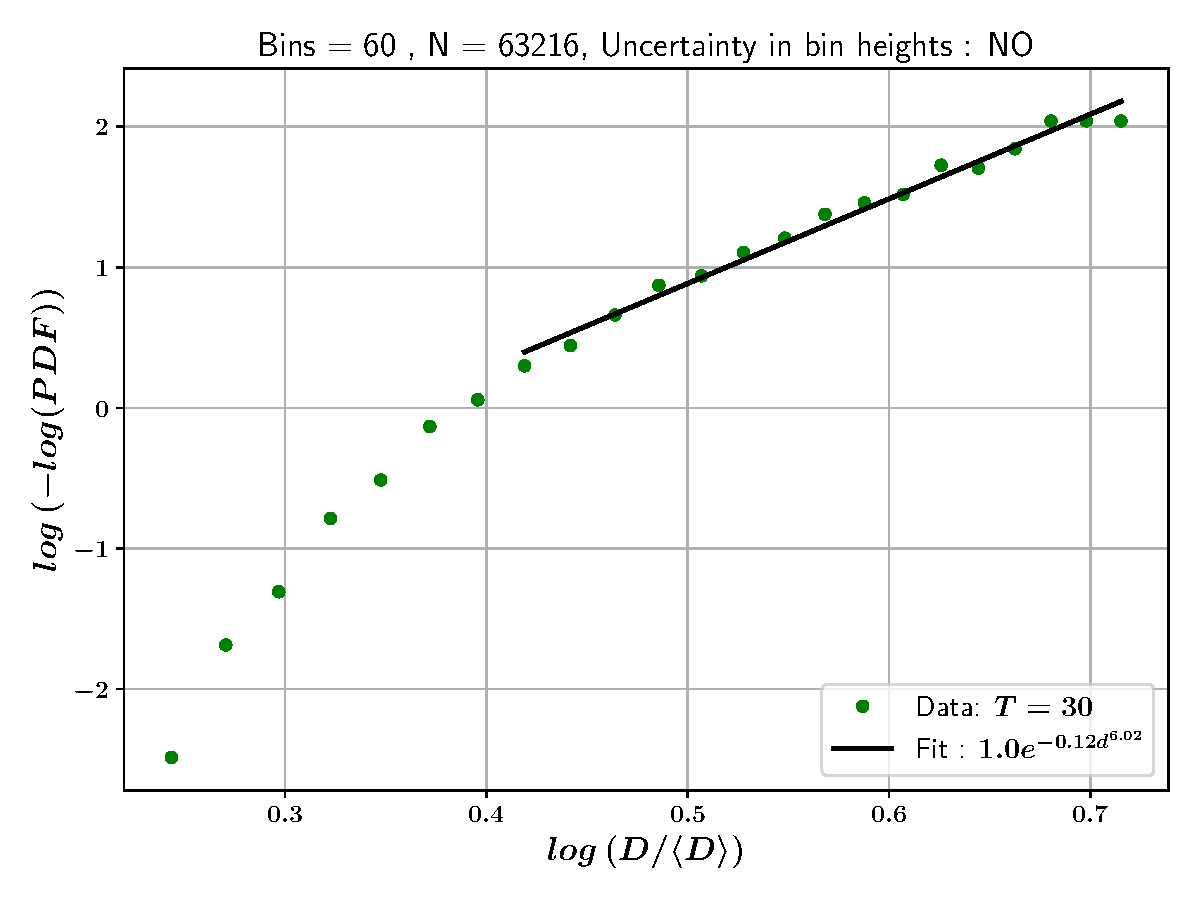
\includegraphics{plots/drop_stats/log_tail_fit_uncertainty_no.pdf} \\
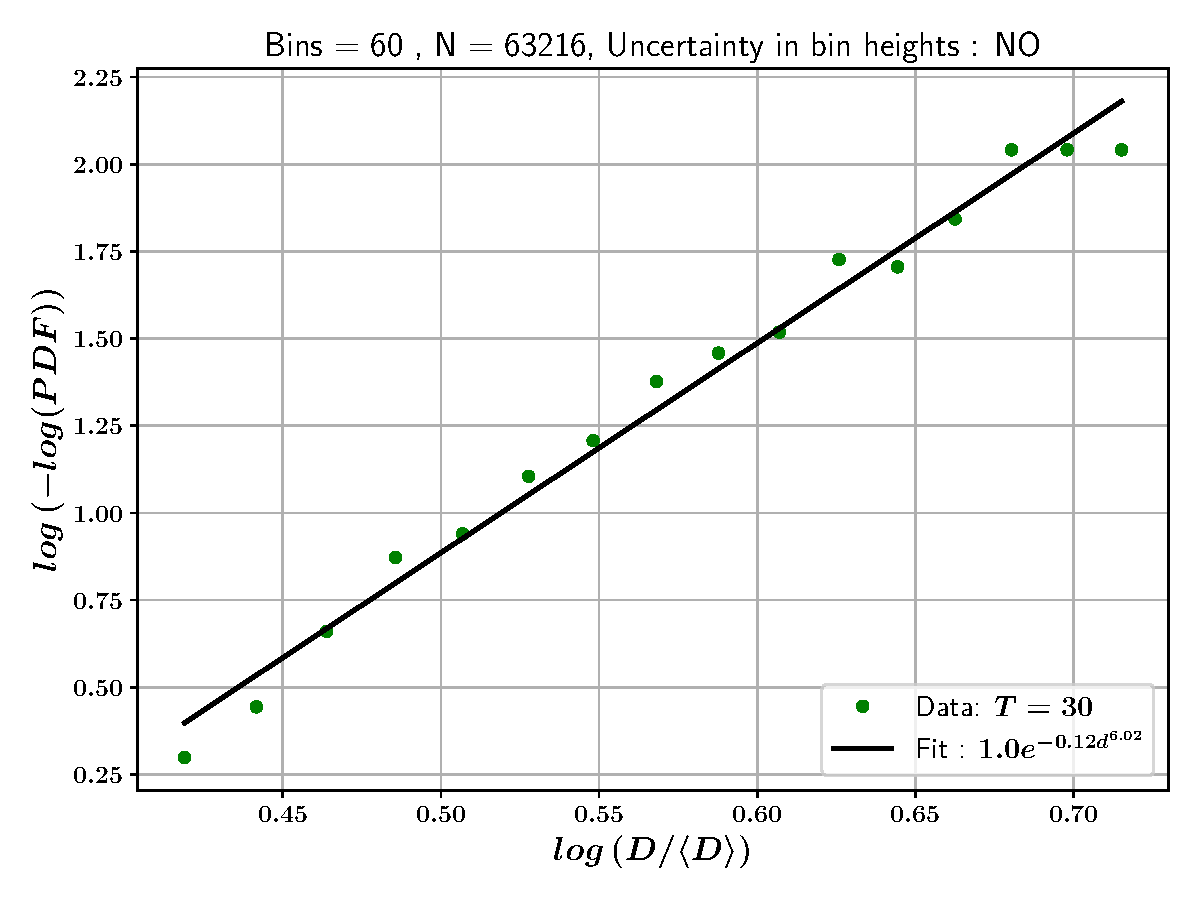
\includegraphics{plots/drop_stats/log_zoom_tail_fit_uncertainty_no.pdf} \\ 
\caption{\blindtext}
\label{log_fits_wo}
\end{figure}


% with uncertainty

\begin{figure}
\centering
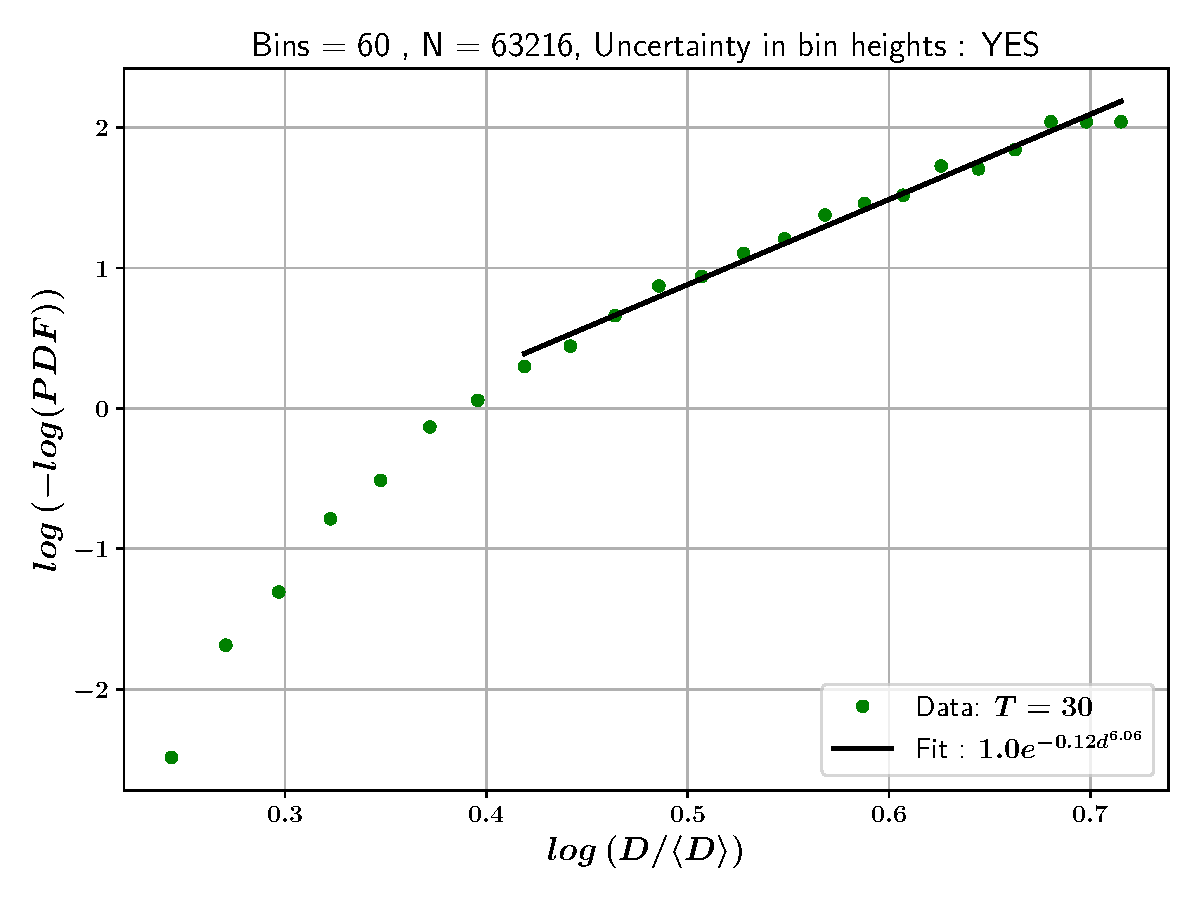
\includegraphics{plots/drop_stats/log_tail_fit_uncertainty_yes.pdf} \\
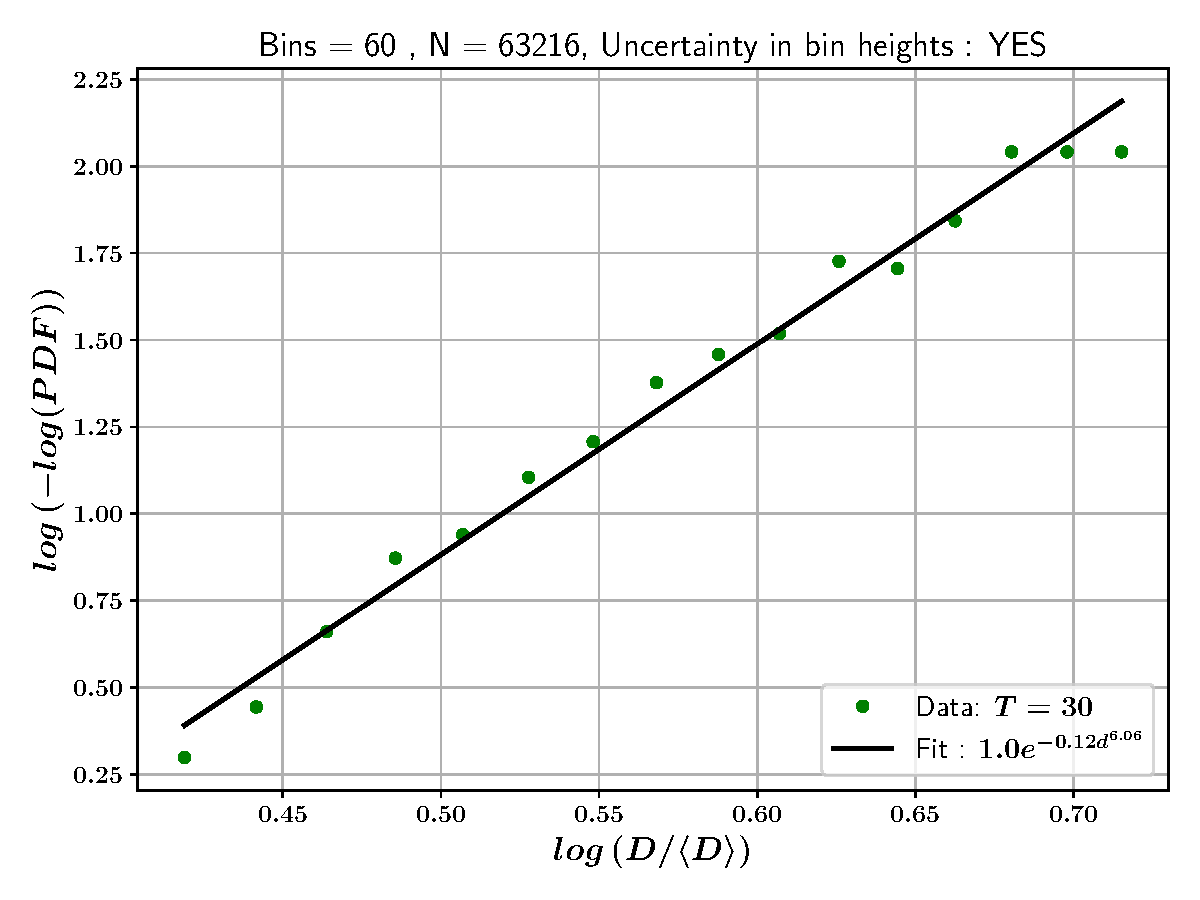
\includegraphics{plots/drop_stats/log_zoom_tail_fit_uncertainty_yes.pdf} \\ 
\caption{\blindtext}
\label{log_fits_with}
\end{figure}

\subsection*{Weakly Non-Linear Theory}



% stephane's predictions and verifications


